\documentclass[a4paper, parskip=full]{scrartcl}
\usepackage[top=3cm, bottom=3.5cm, left=3cm, right=3cm]{geometry}
\usepackage[utf8]{inputenc} % use utf8 file encoding for TeX sources
\usepackage[LGR,T1]{fontenc}    % avoid garbled Unicode text in pdf
\usepackage[german]{babel}  % german hyphenation, quotes, etc
\usepackage{graphicx}       % provides commands for including figures
\usepackage{csquotes}       % provides \enquote{} macro for "quotes"
\usepackage{hyperref}       % detailed hyperlink/pdf configuration
\usepackage{color}
\usepackage{tabu}			% provides tables
\usepackage[nonumberlist]{glossaries}     % provides glossary commands
\hypersetup{                % ‘texdoc hyperref‘ for options
  pdftitle={Pflichtenheft},
  pdfauthor={Nils Prommersberger, Janik Hofmann, Lukas Schmidt, Paul Schillinger, 
  Julius Haag},
    bookmarks=true,
}
\graphicspath{{./figures/}} % Setting the graphicspath

\newcounter{counter}[section]
\setcounter{counter}{10}

\newcommand{\textgreek}[1]{\begingroup\fontencoding{LGR}\selectfont#1\endgroup} % greek letters

% new environment for listing requirements/product data/... with a counter
% example: \begin{Kriterien}{FA} \item[example1] hello \item[example2] world \end{Kriterien}
% output: \textbf{FA 10 example1} \\ hello \\ \textbf{FA 20 example2} \\world
\newenvironment{Kriterien}[1]{
	\let\olditem\item \renewcommand\item[1][]{\olditem[/#1\thecounter /] \textbf{##1} \hfill \\
	\addtocounter{counter}{10}} \begin{description}}
	{\end{description}}


\newcommand{\name}{\textit{QuafelWeb} } % name of product

\title{Pflichtenheft}
\author{Nils Prommersberger, Janik Hofmann, Lukas Schmidt, Paul Schillinger, Julius Haag}
\makeatletter

\definecolor{mintgreen}{RGB}{50,161,137}

% Kopf- und Fußzeilen
\usepackage[automark,
autooneside=false,headsepline=0.5pt,footsepline=0.5pt]{scrlayer-scrpage}
\addtokomafont{headsepline}{\color{mintgreen}}
\addtokomafont{footsepline}{\color{mintgreen}}
\addtokomafont{pagehead}{\normalfont}

% Bisherige Einstellungen für Kopf- und Fußzeilen löschen
\clearpairofpagestyles

% Auf der linken Seite den Dokumentnamen, auf der rechten die aktuelle Section anzeigen
\ihead{\@title}
\ohead{\rightmark}

% Zentriert die Seitenzahl ausgeben
\cfoot*{\pagemark}

% Glossareinträge laden
\makenoidxglossaries
\loadglsentries{./chapters/Glossareintraege}

\begin{document}

% beginn content
\begin{titlepage}
  \centering
  
\includegraphics[width=0.5\linewidth]{KITLogo.png}\par\vspace{1cm}
  	{\scshape \bfseries Scientific Computing Center (SCC) \par}
  	\vspace{0.25cm}
  	{\scshape Melvin Strobl\\Eileen Kühn\par}
  	\vspace{1.5cm}

    {\scshape \Large \bfseries \@title{}: QuafelWeb\par}
    \newcommand{\HRule}{\rule{\linewidth}{0.5mm}}
    {\color{mintgreen}\HRule} \\[0.4cm]
  	{\huge \bfseries \LARGE Webservice zur Einsicht und Verwaltung von Quantensimulationsdaten\par}
    {\color{mintgreen}\HRule} \\[1cm]
  	\vspace{2cm}
  	{\scshape \Large Nils Prommersberger\\Janik Hofmann\\Lukas Schmidt\\Paul Schillinger\\Julius Haag\par}
  	\vfill

\end{titlepage}


\tableofcontents
\section{Vorwort}

Dieses PSE Projekt, hat als Ziel die Erstellung einer Webplatform \name, 
welche genutzt werden kann um die Performance verschiedener Quantensimulatoren 
mit Anschluss and das Quafel Framework, unter verschiedensten Eingabeparametern und 
Hardwareveraussetzungen graphisch darzustellen.

Die Nutzung der Webplatform, besteht in dem Vergleich verschiedener Simulatoren, 
durch die Darstellung der Simulationsdurchläufe gegeneinander, sodass die 
Simulatoren einfach unter verschiedenen Metriken verglichen werden können,
sowie ein seperaten Admin bereich, in welchem authorisierte Benutzer, 
privilegierte Aktionen wie die submittierung neuer Simulationsaufträge and das Quafel Framework,
die Konfiguration der Datendarstellung und die authorisierten Benutzer verwalten kann.

Serverseitig, soll dass Program eine Datenbank führen um die Daten aller bereits durchgeführten 
Simulationen zu speichern. Neue Durchgänge werden auch über die Server Seite an das 
Simulationsframework weiter geleitet, welche die Daten der durchgeführten Simulationsdurchläufe 
für die Serverapplikation bereit stellt.


\section{Zielbestimmung}
Das erklärte Ziel von \name ist es, das Einsehen und vergleichen von Quantensimulatoren mit dem Framework Quafel zu vereinfachen und die Datenspeicherung der bereits durchgeführten Simulationsdurchgänge zu zentralisieren. 
Die Webplatform soll öffentlich zugänglich gemacht werden, um es Forschern weltweit zu ermöglichen auf diese Datensätze zuzugreifen.
Zudem soll das Erstellen neuer Datensätze übersichtlicher und vereinfacht auf einer Website möglich sein, zudem wird sichergestellt das bereits gesammelte Daten nicht noch einmal erstellt werden um somit Zeit und Rechenleistung zu sparen.  



\subsection{Musskriterien}
\setcounter{counter}{10}
\subsubsection{Backend}
\begin{Kriterien}{MK}

    \item Es gibt zu jedem Zeitpunkt mindestens einen Administrator.

    \item Jeder Administrator kann sich ab- und anmelden. 
    
	\item Jeder Administrator weitere Administratoren hinzufügen, oder entfernen.

	\item Jeder Administrator kann über eine graphische Oberfläche Simulationsdurchgänge beauftragen.

    \item Bereits berechnete Simulationsdurchgänge, werden nicht noch einmal berechnet, sondern direkt aus der Datenbank geladen.

	\item Jeder Admin kann über eine graphische Oberfläche neue Hardware Profile erstellen.  

    \item Die Simulationsdurchgänge werden mit dem Framework Quafel erstellt.

    \item Die Daten der Simulationsdurchgänge werden von einer Datei durch das Program eingelesen und verarbeitet.

    \item Die Benutzeroberfläche wird einheitlich in Englisch gehalten.
 
	\item Benchmarkprofile werden nach Hardware, Simulator und Version kategorisiert.

    
	\item Die Anmeldung eines Administrators erfolgt über eine Login Website.
 
    
\end{Kriterien}
\subsubsection{Frontend}
\begin{Kriterien}{MK}

    
	\item Der Webdienst sowie die Datenbank laufen auf einem Rechner.

	\item Die Schnittstelle des \gls{Simulationsbenchmarkprograms} wird von \name verwendet.

	\item Die Daten werden alle auf einer \gls{Datenbank} gespeichert.

	\item Die Weboberfläche ist nur über \gls{HTTPS} verfügbar.

	\item Die Nutzer können das \gls{Frontend} über das Internet abrufen.

	\item Das Frontend übermittelt die Eingabe an das Backend.

	\item Über das Frontend können Benchmark Daten die bereits erfasst wurden durch Graphen eingesehen und verglichen werden.

	\item Das Frontend erlaubt die Angezeigten Daten zu filtern.
 
    \item Graphen müssen als Funktionsgraphen TODO dargestellt werden 

\end{Kriterien}


\newpage
\subsection{Kannkriterien}
\setcounter{counter}{10}
Die folgenden Kannkriterien sind nach absteigender Priorität geordnet.
\subsubsection{Frontend}
\begin{Kriterien}{KK}

	\item Persistente Links TODO.

	\item Die angezeigten Graphen können heruntergeladen werden.

	\item Für die Kommentarfunktion können Vorlagen verwendet werden.

	\item Graphen können zusätzlich als Heatmap dargestellt werden.

	\item Nutzer können Daten Uploaden, welche durch Admins in das System eingebunden werden können.

	\item Administratoren können über eine graphische Oberfläche weitere Administratoren hinzufügen.

    \item Weitere Sprachen können hinzugefügt werden

    
	\item Der Status der submitierten Simulationen wird auf einer separaten Seite im Admin Bereich angezeigt.

\end{Kriterien}


\subsection{Abgrenzungskriterien}
\setcounter{counter}{10}
\subsubsection{Frontend}
\begin{Kriterien}{AK}

	\item Daten der Simulationsdurchgänge können nur überschrieben nicht gelöscht werden 

	\item Die Registrierung neuer Nutzer über das \gls{System} ist nicht möglich.

	\item Nur Authentifizierte Admins können das Admin Panel benutzen.


	\item Ein Endpunkt mit Aufträgen, die sich in Bearbeitung befinden, kann nicht entfernt oder geändert werden.

	\item Werden mehrere Dateien in einem Auftrag hochgeladen, werden sie mit einer Signatur signiert. Es ist nicht möglich, die Dateien einzeln zu signieren bzw. nicht zu signieren.
\end{Kriterien}

\subsubsection{Backend}
\begin{Kriterien}{AK}

	\item Das Backend übernimmt keinen Teil der Simulation.

\end{Kriterien}



\section{Produkteinsatz}
\subsection{Anwendungsbereiche}
Die  Verwendung der Hauptseite von \name soll so offen wie möglich gehalten werden, die Datensätze können somit einer breiten Anzahl an Nutzern, in möglichst informativer aber simpler Form dargestellt werden. Das Admin Panel des Programs soll jedoch nur von berechtigten Personen genutzt werden können, um Sicherheit der verwendeten Systeme, wie auch die Reinheit der Daten zu gewährleisten.

\subsection{Zielgruppe}
Die Zielgruppe der Hauptseite, ist nicht beschränkt, hauptsächlich richtet es sich jedoch an Forschenden im Bereich Quantenrechnern, diese können auf dieser Seite, die Daten nach verschiedenen Parametern Filtern und diese dann als Graph darstellen, es wird auch möglich sein verschiedene Graphen von unterschiedlichen Simulatoren aber mit gleichen Simulationsparametern zu vergleichen und somit Schlüsse auf die Performance der verschiedenen Systeme zu ziehen. In dem Admin Bereich ist es authorisierten Nutzern möglich weitere Simulationen zu konfigurieren und dann auszuführen. Auch die Benutzerverwaltung von weiteren Admins wird auf dieser Seite möglich sein.  

\subsection{Betriebsbedingungen}
Das \gls{System} wird überwiegend in Forschungseinrichtungen eingesetzt. Das System soll rund um die Uhr wartungsfrei bei unbeaufsichtigtem Betrieb zur Verfügung stehen.

\section{Produktumgebung}
\subsection{Hardware}
Das \gls{Frontend} und \gls{Backend} kann von einem \gls{Server} bereitgesetellt werden, welcher folgende Mindestanforderungen erfüllt:
\begin{itemize}
    \item Ausreichende Rechen- und Speicherkapazität für vorgesehene \gls{Nutzer}zahl, Software und \gls{Datenbank}
    \item Im KIT Netz erreichbar
    \item Zugriffsmöglichkeit auf die Simulationsbenchmarkprogramme Server
\end{itemize}
      
Für den Zugriff auf das Frontend und Backend wird ein Computer mit Betriebssystem benötigt, der an das KIT Netz angeschlossen ist.
\subsection{Software}
\subsubsection{Webdienst}
Der Webdienst von \name benötigt:
\begin{itemize}
    \item Linux-Distribution, vorzugsweise Debian basiert
    \item Relationale Datenbank: postgresql
    \item Python 3
    \item Django mit zugehörigen Abhängigkeiten
\end{itemize}

\subsubsection{Frontend und Backend}
Serverseitig ist für den Betrieb des Frontends und Backends nötig:
\begin{itemize}
    \item Linux-Distribution, vorzugsweise Debian basiert
    \item Apache 2
\end{itemize}
\gls{Client}seitig werden folgende Browser unterstützt:
\begin{itemize}
    \item Safari ab Version 11
    \item Chrome ab Version 69
    \item Firefox ab Version 57
\end{itemize}

\subsection{Orgware}
Ein reibungsloser Betrieb kann nur unter nachstehenden Bedingungen erfolgen:
\begin{itemize}
    \item unterbrechungsfreie Netzwerkverbindung
    \item Verfügbarkeit eines \glslink{Administrator}{Administrators}, der Erstkonfiguration und \gls{Endpunkt}verwaltung im Backend vornimmt
    \item mindestens ein Simulator TODO.
\end{itemize}


\section{Funktionale Anforderungen}
\setcounter{counter}{10}
\subsection{Frontend}
\begin{Kriterien}{FA}

    \item[Aufteilung] Die Website ist in zwei grobe Teile aufgeteilt. Den Benutzerbereich, den alle einsehen können und der für die Veranschaulichung von Daten verantwortlich ist und den Administratorbereich, der für die Verwaltung der Benutzer, Hardwareprofile und das Submittieren von Daten genutzt wird.

    \item[Benutzerbereich] Der Benutzerbereich besteht aus 

\end{Kriterien}
\paragraph{Benutzerbereich}
\begin{Kriterien}{FA}
    
    \item[Farben der Grafen] Die Grafen werden zur Übersichtlichkeit in unterschiedlichen Farben dargestellt.

    \item[Auswahl der Simulatoren] Die Simulatoren können nach Hardwareprofil, Simulationsprogramm und Version gefiltert und zum Vergleich ausgewählt werden.

    \item[Entfernen der Simulatoren] Die Simulatoren können aus dem Vergleich wieder entfernt werden.

    \item[Auswahl des Plots] Zur Veranschaulichung durch Grafen stehen folgende Datenpunkte zur Verfügung: Anzahl an Shots, QBits, Evaluations und die Tiefe der Schaltungen. Es kann bei der Darstellung durch Funktionsgrafen jeweils nur eines dieser Dinge ausgewählt sein. TODO

    \item[Auswahl der Spanne] Die Spanne auf der der Graf dargestellt werden soll kann nur für den ausgewählten Datenpunkt eingestellt werden.

    \item[Beschränkung des Plots] Es werden nur Daten als Grafen dargestellt, die zur Verfügung stehen. Daten, die noch nicht erstellt wurden, können von Benutzern nicht als Plot eingestellt werden.



    \item[Anmelden] Ein registrierter Administrator kann sich über Chibotle mit seinem KIT-Account anmelden. 

    \item[Abmelden] Ein angemeldeter Administrator kann sich abmelden.

    \item[Registrieren] Ein angemeldeter Administrator kann einen anderen Administrator registrieren. 
    


    \item[Erstellung von Harwareprofilen] Ein Administrator kann neue Hardwareprofile erstellen und konfigurieren. Sobald für dieses Hardwareprofil Daten bestehen, wird dieses und die darauf laufenden Simulationsprogramme den Benutzern zur Auswahl zur Verfügung gestellt.

    \item[Entfernen von Hardwareprofilen] Ein Administrator kann Hardwareprofile löschen. Diese und alle darauf laufenden Simulationsprogramme werden den Benutzern dann nicht mehr zur verfügung gestellt.



    \item[Submittieren von Simulationsdaten] Ein Administrator kann neue Simulationsdaten erstellen lassen. Dabei kann er sich entscheiden ob schon erstellte Daten überschrieben werden sollen oder nicht.

    \item[Submittieren filtern] Ein Adminisrator kann filtern, für welche Simulationsprogramme auf welchen Hardwareprofilen mit welcher Version neue Simulationdaten erstellt werden sollen.

    \item[Submittieren konfigurieren] Ein Administrator kann einstellen in welcher Spanne er welche Daten erstellen möchte.

    \item[Schon erstellte Daten] Wenn ein Administrator jegliche Spannen konfiguriert hat, wird für jedes ausgewählte Simulationsprogrammprofil die Anzahl der schon erzeugten Daten angezeigt.

\end{Kriterien}

\subsection{Backend}
\begin{Kriterien}{FA}

    \item[HTTPS-Forward] Versucht ein Benutzer über HTTP auf die Website zuzugreifen, wird er auf HTTPS umgeleitet.

    \item[Startseite] Wir die Website ohne eine spezifischen Pfad aufgerufen, so wird auf das Datenpanel umgeleitet.

	\item[Prüfung von Anfragen] Das Backend prüft Anfragen von \glslink{Client}{Clients} auf Zugriffsberechtigung.

    \item Die Simulationsdurchgänge werden über ssh auf dem entsprechenden Server gestartet.

	\item[Admin-Anmeldung] Meldet sich ein \gls{Administrator} an, wird die Admin-Übersicht angezeigt.

	\item[Erstellen eines Auftrags] Das Backend prüft die Gültigkeit eines erstellten Simulationsauftrags und sendet diesen an den entsprechenden Server.



\end{Kriterien}


\paragraph{Kannkriterien}

\begin{Kriterien}{FA}

	\item[Einrichtungsprozess] Es gibt einen Einrichtungsprozess für die Inbetriebnahme von \textit{Argos}.
	
	\newpage

	\item[Kommentarfunktion] Der Administrator kann für einen neuen Endpunkt die Kommentarfunktion erlauben. Einem signierenden Nutzer wird ein zusätzliches Textfeld angezeigt, das er ausfüllen kann. Der Inhalt des Textfeldes wird an den Ersteller des Auftrags weitergeleitet.

	\item[Erfolgte Signatur] Der Administrator kann eine Aktion bei einer erfolgten Signatur festlegen.

	\item[Auftragsgenehmigung] Der Administrator kann eine Aktion beim Abschluss eines Auftrags dieses Endpunktes festlegen.


\end{Kriterien}

\subsection{Frontend}
\begin{Kriterien}{FA}

	\item[Nutzer-Login] Beim Öffnen der Webseite wird der Anmeldebereich angezeigt. Der Nutzer kann sich hier mit seinen Anmeldedaten anmelden.

	\item[Abmelden] Klickt der Nutzer auf den Menüpunkt \enquote{Abmelden}, erscheint die Anzeige \enquote{erfolgreich abgemeldet} und der Nutzer wird zum Anmeldebereich weitergeleitet.

	\item[Nutzer-Startseite] Auf der Startseite des Frontends sind alle vom Nutzer erstellten Aufträge gelistet. Diese können nach den Kriterien Auftrags-ID, Auftragsname, \gls{Status} oder Erstellungsdatum sortiert werden.

	\item[Seite: Zu signierende Aufträge] Auf der Seite für \enquote{Zu signierende Aufträge} des Frontends sind alle Aufträge gelistet, die der Nutzer mit seinen Rollen signieren kann. Diese können nach Priorität/Datum/Name sortiert werden.

	\item[Detailansicht (selbst erstellte Aufträge)] Beim Klicken auf das
	\enquote{Auge}-Symbol neben einem selbst erstellten Auftrag werden die
	folgenden Details des Auftrags angezeigt: Status,
	Ersteller, Erstellungsdatum, Datum der letzten Änderung, Auftragsverlauf,
	zugehörige Formulardaten und Dateien.  Es werden die Buttons \enquote{Download} und
	\enquote{Zurückziehen} angezeigt.

	\item[Detailansicht (zu signierende Aufträge)] Beim Klicken auf einen
	zu signierenden Auftrag werden auf einer neuen Seite angezeigt:
	Status, Ersteller, Erstellungsdatum, Datum der letzten Änderung,
	Auftragsverlauf, zugehörige Formulardaten und Dateien. Es werden die Buttons
	\enquote{Signieren} und \enquote{Auftrag ablehnen} angezeigt.

	\item[Download von Dateien] Beim Klicken auf den \enquote{Download}-Button eines Auftrags werden die zugehörigen Dateien heruntergeladen.

	\item[Signieren] Je nach definierter Art kann die Signatur eines Auftrags erst nach Download der zugehörigen Dateien erfolgen. Ein Nutzer kann einen Auftrag nur ein Mal signieren.

	\item[Ablehnen eines Auftrags] Der Nutzer kann durch das Klicken des \enquote{Auftrag ablehnen}-Buttons, der in der Detailansicht des jeweiligen Auftrags  angezeigt wird, einen Auftrag ablehnen. Der Auftrag wird als abgelehnt gekennzeichnet und kann nicht mehr signiert oder genehmigt werden.

	\item[Nach der Signatur] Für alle Nutzer mit derselben Rolle wird nach der Signatur der jeweilige Auftrag nicht mehr auf der Seite \enquote{Zu signierende Aufträge} angezeigt. Der signierende Nutzer und andere Nutzer mit derselben Rolle können den Auftrag unter dem Menüpunkt \enquote{Historie} einsehen.


	\item[Benachrichtigung im Frontend] Ändert sich der Status eines erstellten Auftrags (ein Nutzer hat den Auftrag signiert, der Auftrag wurde abgelehnt) oder muss der Nutzer selbst einen Auftrag signieren, wird dies im Frontend unter dem Menüpunkt \enquote{Benachrichtigungen} angezeigt.

	\item[Benachrichtigung per E-Mail] Ein Nutzer kann über die Nutzereinstellungen im Frontend die Benachrichtigung per E-Mail an- und ausschalten. Eine Benachrichtigungs-E-Mail wird immer an die in den Nutzerdaten gespeicherte E-Mail-Adresse gesendet.

	\item[Erstellung von Aufträgen] Beim Klicken auf einen der Endpunkte, die im Menü des Frontends gelistet sind, wird der Nutzer zu einer Erstellungsansicht weitergeleitet.
	Die vom Nutzer auszufüllenden Informationen hängen vom gewählten Endpunkt ab. Der \enquote{Erstellen}-Button ist zunächst ausgegraut. Hat der Nutzer alle Pflichtfelder ausgefüllt, kann er den \enquote{Erstellen}-Button klicken.

	\item[Bestätigungs-E-Mail] Hat ein Nutzer einen Auftrag erstellt, so erhält er eine Bestätigungs-E-Mail mit Details zu seinem Auftrag.
		
	\item[Hochladen von Dateien] Beim Klicken auf den \enquote{Upload}-Button bei der Auftragserstellung wird ein Datei-Upload-Dialog angezeigt und der Nutzer kann ein oder mehrere Dateien auswählen, die hochgeladen werden.

	\item[Verarbeitung von hochgeladenen Dateien] Das \gls{System} sammelt Metadaten von hochgeladenen Dateien, wie Größe, Zeitstempel und Hashwert, und zeigt diese in der Detailansicht des jeweiligen Auftrags an.
	
	\newpage

	\item[Genehmigung von Aufträgen] Haben alle benötigten Rollen den Auftrag signiert, ist er genehmigt. Der Ersteller des Auftrags wird benachrichtigt.

	\item[Zurückziehen von Aufträgen] Ist ein Auftrag noch nicht genehmigt (es haben noch nicht alle nötigen Rollen signiert), kann der Auftragsersteller diesen zurückziehen, indem er auf den \enquote{Zurückziehen}-Button der Detailansicht des jeweiligen Auftrags klickt und das Zurückziehen bestätigt.

	\item[Löschen von abgelehnten Aufträgen] Ein abgelehnter Auftrag kann vom Ersteller gelöscht werden.

	\item[Löschen von genehmigten Aufträgen] Das Löschen von genehmigten Aufträgen ist je nach Endpunktkonfiguration möglich.

\end{Kriterien}

\paragraph{Kannkriterien}

\begin{Kriterien}{FA}

	\item[Tooltip Text] Beim Überfahren auszufüllender Felder werden zusätzliche Informationen eingeblendet.

	\item[Aufträge sortieren] Aufträge auf der Nutzer-Übersicht können nach Priorität/Datum/Name sortiert werden.

	\item[Mobile Endgeräte] Das Frontend ist für mobile Endgeräte optimiert.

	\item[\gls{Wiki}] Es steht ein Wiki zur Verfügung, in dem Informationen zur Konfiguration und Benutzung aufgeführt sind.



\end{Kriterien}

\section{Produktdaten}
\label{sec:data}
\setcounter{counter}{10}
\begin{Kriterien}{PD}
\item[\gls{Nutzer}daten] Folgende Nutzerdaten werden gespeichert:
\end{Kriterien}
\vspace{-10pt}
\begin{itemize}\itemsep-10pt
\item Name, Vorname
\item E-Mail-Adresse
\item eindeutige Nutzer-ID
\item vom \gls{LDAP} festgelegte \glspl{Rolle}
\item Ein-/Ausschalten der E-Mail-Benachrichtigung
\end{itemize}


\begin{Kriterien}{PD}
\item[\gls{Administrator}daten] Folgende Administratordaten werden gespeichert:
\end{Kriterien}
\vspace{-10pt}
\begin{itemize}\itemsep-10pt
\item Name, Vorname
\item E-Mail-Adresse
\item Passwort in verschlüsselter Form
\end{itemize}


\begin{Kriterien}{PD}
\item[\gls{Endpunkt}] Für jeden definierten Endpunkt werden folgende Kriterien gespeichert:
\end{Kriterien}
\vspace{-10pt}
\begin{itemize}\itemsep-10pt
\item Name des Endpunkts
\item Eindeutige Endpunkt-ID
\item \gls{Modus} des Endpunkts (parallel/sequentiell)
\item Anzahl der benötigten \glspl{Signatur}
\item Rollen, die signieren müssen
\item Nutzer, die signieren müssen
\item Bei sequentiellem Modus: Reihenfolge der signierenden Rollen/Nutzer
\item Ein-/Ausschalten der E-Mail-Benachrichtigung für Nutzer, deren Signatur benötigt wird
\item \gls{Formular}zusammensetzung
\end{itemize}

\begin{Kriterien}{PD}
\item[\gls{Auftrag}] Jeder Auftrag wird mit folgenden Informationen gespeichert:
\end{Kriterien}
\vspace{-10pt}
\begin{itemize}\itemsep-10pt
\item ID des verwendeten Endpunkts
\item Eindeutige Auftrag-ID
\item Nutzer-ID des Erstellers
\item Erstellungsdatum
\item Benötigte Signaturen
\item Nutzer-ID erfolgter Signaturen mit Zeitstempel
\item Bei sequentiellem Modus: Reihenfolge der Signaturen
\item Ausgefülltes Formular mit zugehörigen Dateien
\end{itemize}

\begin{Kriterien}{PD}
\item[Datei] Für jede hochgeladene Datei werden folgende Metadaten über die Datei gespeichert:
\end{Kriterien}
\vspace{-10pt}
\begin{itemize}\itemsep-10pt
\item Autor
\item Größe
\item Zeitstempel
\item Hashwert
\end{itemize}

\section{Nichtfunktionale Anforderungen}
\setcounter{counter}{10}
\subsection{Webdienst}
\begin{Kriterien}{NA}

	\item[Archivgröße] Es können bis zu 10.000 \glspl{Auftrag} verwaltet werden.

	\item[Anzahl Aufträge] Es können sich bis zu 1.000 Aufträge in Bearbeitung befinden.

	\item[Dateigröße] Die standardmäßig festgelegte Grenze für die Größe einer hochzuladenden Datei liegt bei 20 MB.

	\item[Anzahl \gls{Nutzer}] Das \gls{System} kann mit bis zu 10.000 Nutzern umgehen.

	\item[Verlässlichkeit] Das System darf nicht öfter als einmal pro Woche ausfallen.

	\item[Zugriff] Bis zu 100 \glspl{Client} können gleichzeitig auf den \gls{Webdienst} zugreifen.

	\item[Zugriffsschutz] Hochgeladene Dateien werden auf dem \gls{Server} nicht geändert und als \enquote{read-only} gespeichert.

\end{Kriterien}

\subsection{Frontend}
\begin{Kriterien}{NA}

	\item[Übersichtlichkeit] Die Nutzerfreundlichkeit steht im Vordergrund, sodass der Nutzer sich intuitiv zurechtfinden kann. 

\end{Kriterien}

\section{Globale Testfälle}
\newcommand{\stand}{\textbf{Stand: }}
\newcommand{\aktion}{\\ \textbf{Aktion: }}
\newcommand{\ergebnis}{\\ \textbf{Reaktion: }}

\setcounter{counter}{10}
\subsection{Frontend}
\begin{Kriterien}{TF}
%Frontend
    \item[Anmeldung des \glslink{Administrator}{Administrators}]
    \stand Ausgemeldeter Nutzer ist auf Startseite.
    \aktion Ein Administrator klickt auf "Anmelden" und meldet sich über Shibboleth an.
    \ergebnis Der Administrator wird angemeldet und wird zum Adminpanel weitergeleitet.

    \item[Abmeldung des Administrator]
    \stand Ein Administrator ist angemeldet.
    \aktion Ein Administrator meldet sich über das Adminpanel ab.
    \ergebnis Der Administrator wird abgemeldet und landet abgemeldet auf der Graphenseite.

    \item[Entfernung von Administrator]
    \textbf{1. }\stand Es existieren mehr als ein Administratoren.
    \aktion Ein Administrator löscht einen Administrator über das Adminpanel.
    \ergebnis Administrator wird gelöscht.
    
    \textbf{2. }\stand Es existiert nur ein letzter Administrator.
    \aktion Der letzte Administrator versucht sich als Administrator zu löschen.
    \ergebnis Ein Fehler wird angezeigt. Die Rechte des letzten Administrator werden nicht entzogen.
    
    \item[Hinzufügen von Administratoren] 
    \stand Adminpanel ist offen.
    \aktion Ein Administrator fügt einen neuen Administrator über die E-Mail-Adresse hinzu.
    \ergebnis Der Nutzer der E-Mail-Adresse wird als Administrator angelegt.

    \item[Beauftragung Simulationsdurchgänge]
    \stand Die Submitierungsseite ist offen.
    \aktion Administrator wählte Simulationsdurchgänge aus und klickt auf submitieren.
    \ergebnis Client schickt Submitierungsauftrag an den Server.

    \item[Benchmarkprofilerstellung] 
    \stand Die SUbmitierungsseite ist offen. Bestimmte Hardware, Simulationssoftware und Versionen sind ausgewählt. 
    \aktion Ein Administrator drückt auf "Benchmarkprofil speichern".
    \ergebnis Benchmarkprofil wird auf dem Server gespeichert und dem Administrator als neues auswählbares Benchmarkprofil angezeigt.

    \subsection{Backend}
    
    \item[Vorhandene Simulationsdurchgänge laden]
    \stand Submitierungsauftrag mit bereits vorhandenen Simulationsdurchgängen wird vom Server verarbeitet.
    \ergebnis Bereits vorhandene Simulationsdurchgänge in der Datenbank werden geladen anstatt nochmals berechnet zu werden.

    \item[Berechnung Simulationsdurchgänge] 
    \stand Simulationsdurchgänge wurden submitiert.
    \ergebnis Server schickt zu berechnende Simulationsdurchgänge an QUAFEL und wartet auf Ergebnisse.

    \item[Einlesen QUAFEL Ergebnisse]
    \stand QUAFEL schickt Ergebnisse als Datei an den Server.
    \ergebnis Das Backend verarbeitet die Datei. Die Ergebnisse werden in der Datenbank gespeichert und zur Verfügung gestellt.

    


    
    \item[Zugriff über \gls{HTTP}] Der Admin versucht, über HTTP auf das Backend zuzugreifen.\ergebnis Der Admin wird auf \gls{HTTPS} umgeleitet.

    \item[Admin-Übersicht] Korrekte Ansicht der Admin-Übersicht.\ergebnis Der Administrator kann in seiner Admin-Übersicht auf eine Liste aller \glspl{Auftrag}, eine Liste aller \glspl{Endpunkt} und auf den Menüpunkt \enquote{Endpunkt erstellen} zugreifen.

	\item[Endpunkt als auslaufend markieren] Der Administrator markiert im Menüpunkt \enquote{Endpunkte verwalten} einen Endpunkt als auslaufend. \ergebnis Im \gls{Frontend} können keine neuen Aufträge zu diesem Endpunkt erstellt werden.

    \item[Auslaufenden Endpunkt löschen] Alle Aufträge zu einem auslaufenden Endpunkt wurden genehmigt.\ergebnis Der Endpunkt wird nicht mehr angezeigt.

	\item[Erstellung eines neuen Endpunkts] Der Administrator klickt auf den Menüpunkt \enquote{Endpunkt erstellen}. \ergebnis Er wird auf eine neue Seite weitergeleitet. Er kann den Namen und den \gls{Modus} des Endpunkts festlegen. Weiterhin kann er benötigte \glspl{Signatur} von bestimmten \glspl{Rolle} oder konkreten \glslink{Nutzer}{Nutzern} hinzufügen. Er kann den Inhalt eines \glslink{Formular}{Formulars} spezifizieren, das vom Auftragsersteller ausgefüllt werden muss. Sind noch nicht alle Felder ausgefüllt, kann der Administrator den neuen Endpunkt nicht erstellen.

    \item[Nach Erstellung eines neuen Endpunkts] Der Administrator bestätigt die Erstellung eines neuen konfigurierten Endpunkts. \ergebnis In der Liste aller Endpunkte wird ein neuer Eintrag mit den soeben festgelegten Details angezeigt. Im Frontend können Nutzer Aufträge für diesen Endpunkt erstellen.

\end{Kriterien}

\subsection{Backend}
\begin{Kriterien}{TF}

    \item[Anmeldung erfolgreich] Der Nutzer meldet sich mit korrekten Authentifizierungsdaten an.\ergebnis Der Nutzer wird zur Nutzer-Startseite weitergeleitet und als angemeldet vom \gls{System} erkannt.

    \item[Anmeldung fehlgeschlagen] Der Nutzer meldet sich mit falschen Authentifizierungsdaten an.\ergebnis Der Nutzer wird darauf hingewiesen, dass seine eingegebenen Authentifizierungsdaten nicht korrekt sind.

    \item[Abmeldung] Abmeldung eines Nutzers. \ergebnis Der Nutzer bekommt die Bestätigung der erfolgreichen Abmeldung und wird zum Anmeldebereich weitergeleitet.

    \item[Nicht autorisierter Zugriff] Ist der Nutzer nicht angemeldet und versucht, auf geschützte Inhalte zuzugreifen, wird mit einer \enquote{nicht autorisiert}-Meldung reagiert und der Zugriff verweigert.

    \item[Zugriff über HTTP] Der Nutzer versucht, über HTTP auf das Frontend zuzugreifen.\ergebnis Der Nutzer wird auf HTTPS umgeleitet.

    \item[\gls{LDAP} nicht erreichbar] Nutzer greift auf das Frontend zu, falls der LDAP-\gls{Server} nicht erreichbar ist. \ergebnis Der Server meldet sowohl über das Frontend als auch über die \gls{REST-API} einen Authentifizierungsfehler, dass der LDAP-Server nicht erreichbar ist und meldet dem Nutzer, dass der Administrator bereits per E-Mail benachrichtigt wurde.

     \item[Auftrag erstellen] Ein Nutzer konfiguriert zu einem bestimmten Endpunkt einen Auftrag und bestätigt die Erstellung. \ergebnis Der erstellte Auftrag wird unter \enquote{Meine Aufträge} angezeigt. Der Nutzer bekommt alle Auftragsdetails per E-Mail zugeschickt. Die Nutzer mit den Rollen, deren Signatur zuerst benötigt wird, werden benachrichtigt.

      \item[Auftrag signieren] Ein Nutzer signiert einen Auftrag. \ergebnis Für alle Nutzer mit der gleichen Rolle wie die des Signierenden wird der Auftrag nicht mehr unter \enquote{Zu signierende Aufträge} angezeigt. Unter dem Menüpunkt \enquote{Historie} können diese Nutzer den Auftrag einsehen.

\newpage
    \item[Auftrag abgelehnt] Ein Nutzer, dessen Signatur für einen Auftrag benötigt wird, lehnt den Auftrag ab. \ergebnis Der Auftrag wird als abgelehnt gekennzeichnet und kann nicht mehr signiert oder genehmigt werden. Der Ersteller des Auftrags erhält eine Benachrichtigung und kann den Auftrag löschen.

 	\item[\gls{Status}änderung eines Auftrags] Der Status eines Auftrags ändert sich. \ergebnis Der Ersteller des Auftrags wird im Frontend über die Statusänderung benachrichtigt. Abhängig von seiner Nutzereinstellung bekommt er zusätzlich eine E-Mail-Benachrichtigung.

    \item[E-Mail-Benachrichtigungen ausschalten] Ein Nutzer schaltet im Frontend unter dem Menüpunkt \enquote{Einstellungen} die E-Mail-Benachrichtigungen aus. \ergebnis Der Nutzer erhält keine Benachrichtigungen per E-Mail mehr. Die Benachrichtigungen im Frontend werden weiterhin angezeigt.

	\item[Auftrag zurückziehen] Ein Nutzer zieht einen selbst erstellten Auftrag zurück. \ergebnis Der Auftrag kann nicht mehr signiert oder genehmigt werden.

\end{Kriterien}

\section{Systemmodelle}
\subsection{Backend}
\begin{figure}[htbp]
	\centering
	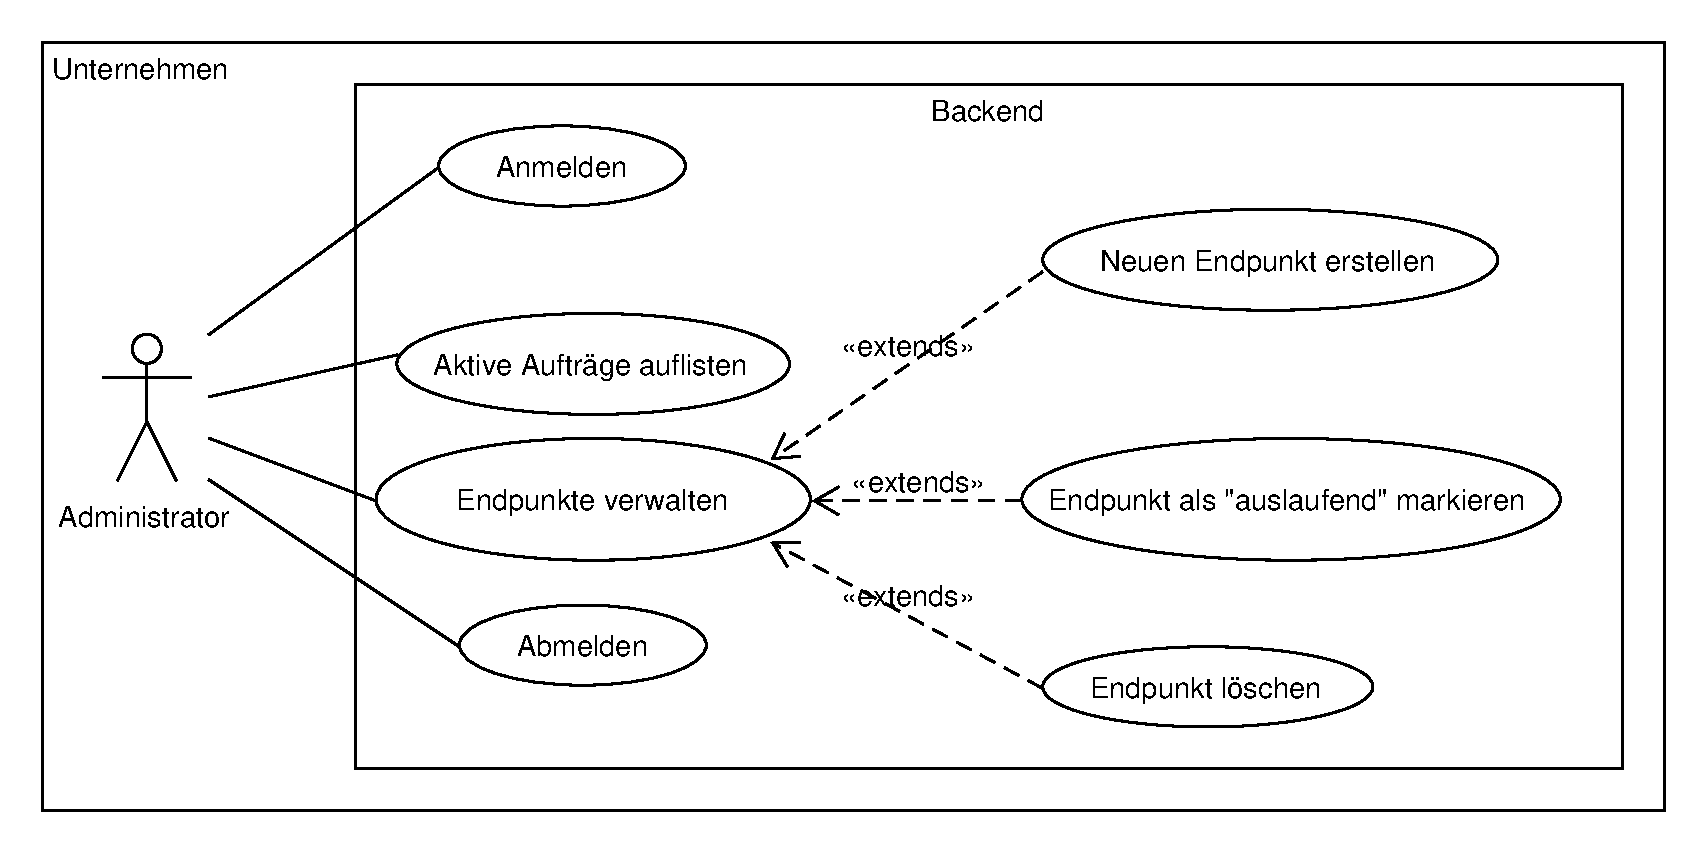
\includegraphics[width=1.0\textwidth]{UseCase_Admin.pdf}
	\caption{Aktionsübersicht des Administrators}
	\label{fig:Bild1}
\end{figure}
\subsubsection{Szenario: Endpunktkonfiguration}
\paragraph{Beschreibung}
Der \gls{Administrator} nimmt die Konfiguration eines neuen \glslink{Endpunkt}{Endpunkts} im bestehenden \gls{System} vor.
Der neue Endpunkt stellt einen neuen Kontext dar, um das Mehr-Augen-Prinzip effizient umzusetzen.
Nach erfolgreicher Konfiguration können die \gls{Nutzer} den Endpunkt nutzen, um einen \gls{Auftrag} in diesem Kontext zu stellen.

\paragraph{Korrekter Ablauf}
Der Administrator hat sich im System angemeldet und befindet sich in der Administratoren-Übersicht des \glslink{Backend}{Backends}.
Er klickt auf den \enquote{Endpunkt erstellen}-Button und wird zu einem \gls{Editor} weitergeleitet.
Dort wählt er den Namen \enquote{Urlaubsantrag} für diesen Endpunkt.
Im Editor findet er eine Vielzahl an Konfigurationselementen. Ein Großteil davon liegt in der Form von Schaltern vor, die Kriterien ein- oder ausschalten. Zu diesen gehören die Benachrichtigung für Auftragserhaltende, die Löschbarkeit eines Auftrags durch den Auftragsersteller, die Art der \gls{Signatur} und ob ein Nutzer weitere Augenpaare hinzufügen kann.  Es besteht die Möglickeit ein \gls{Formular} zu definieren, das vom Auftragsersteller ausgefüllt werden muss. Andere Konfigurationselemente dienen dem Hinzufügen, Entfernen und Spezifizieren der benötigten Signaturen.
Der Administrator konfiguriert den Endpunkt wie folgt:
\begin{itemize}
	\item Anzahl der Augenpaare: vier
	\item sequentieller \glslink{Modus}{Signaturmodus}
	\item \gls{LDAP}-\glspl{Rolle} in entsprechender Reihenfolge: Sekretariat, Personalleitung, Chef
	\item E-Mail-Benachrichtigungen für Auftragserhaltende sind deaktiviert.
	\item Eine Signatur wird durch Klicken eines Bestätigungsbuttons erfüllt.
	\item Ein Auftrag, der abgelehnt wurde, kann vom Auftragssteller gelöscht werden.
	\item Der Auftragssteller erhält eine Benachrichtigung, wenn sein Auftrag genehmigt wurde.
\end{itemize}
Der Administrator bestätigt diese Konfiguration durch Klicken auf den \enquote{Erstellen}-Button.
Er wird auf die Startseite des Backends weitergeleitet.
Angemeldete Nutzer sehen einen neuen Endpunkt in der Endpunktauflistung und können diesen nutzen.

\paragraph{Abgebrochener Ablauf}
Der Administrator bricht die Endpunktkonfiguration an beliebiger Stelle durch Klicken des \enquote{Abbrechen}-Buttons ab.

\subsubsection{Szenario: Endpunkt entfernen}
\paragraph{Beschreibung}
Aufgrund einer Änderung der Firmenpolitik müssen nun alle wichtigen, die Firma betreffenden Anträge nicht mehr nur vom CEO (Chief Executive Officer), sondern auch vom CFO (Chief Financial Officer) signiert werden. Deshalb muss der bereits bestehende Endpunkt \enquote{Wichtige Anträge} entfernt werden und durch einen neuen  mit Berücksichtigung der Signatur des CFO erstellt werden.
\paragraph{Korrekter Ablauf}
Dazu klickt der bereits angemeldete Administrator in der Administratorübersicht auf den Menüpunkt \enquote{Endpunkt entfernen}. Der Administrator wird gebeten, den zu entfernenden Endpunkt auszuwählen. Er wählt den Endpunkt \enquote{Wichtige Anträge} aus und klickt auf \enquote{Endpunkt entfernen}. Dem Administrator wird der Hinweis angezeigt, dass Endpunkte erst dann entfernt werden können, wenn alle aktiven Aufträge fertiggestellt sind. Da noch immer aktive Aufträge laufen, wird der Administrator gefragt, ob er den Endpunkt als \enquote{auslaufend} markieren möchte. Er muss bestätigen, dass nun keine neuen Aufträge für diesen Endpunkt angenommen werden können. In seiner Ansicht wird nun unter dem Menüpunkt \enquote{Endpunkte verwalten} der Name des Endpunkts \enquote{Wichtige Aufträge} ausgegraut angezeigt.
Er konfiguriert den neuen Endpunkt und meldet sich vom Backend ab.
\paragraph{Abgebrochener Ablauf}
Falls der Administrator das Fenster schließt, nicht auf den \enquote{Endpunkt löschen}-Button drückt oder das Löschen nicht bestätigt, wird die Löschung des Endpunkts nicht vorgenommen.


\subsection{Frontend}
\begin{figure}[htbp]
	\centering
	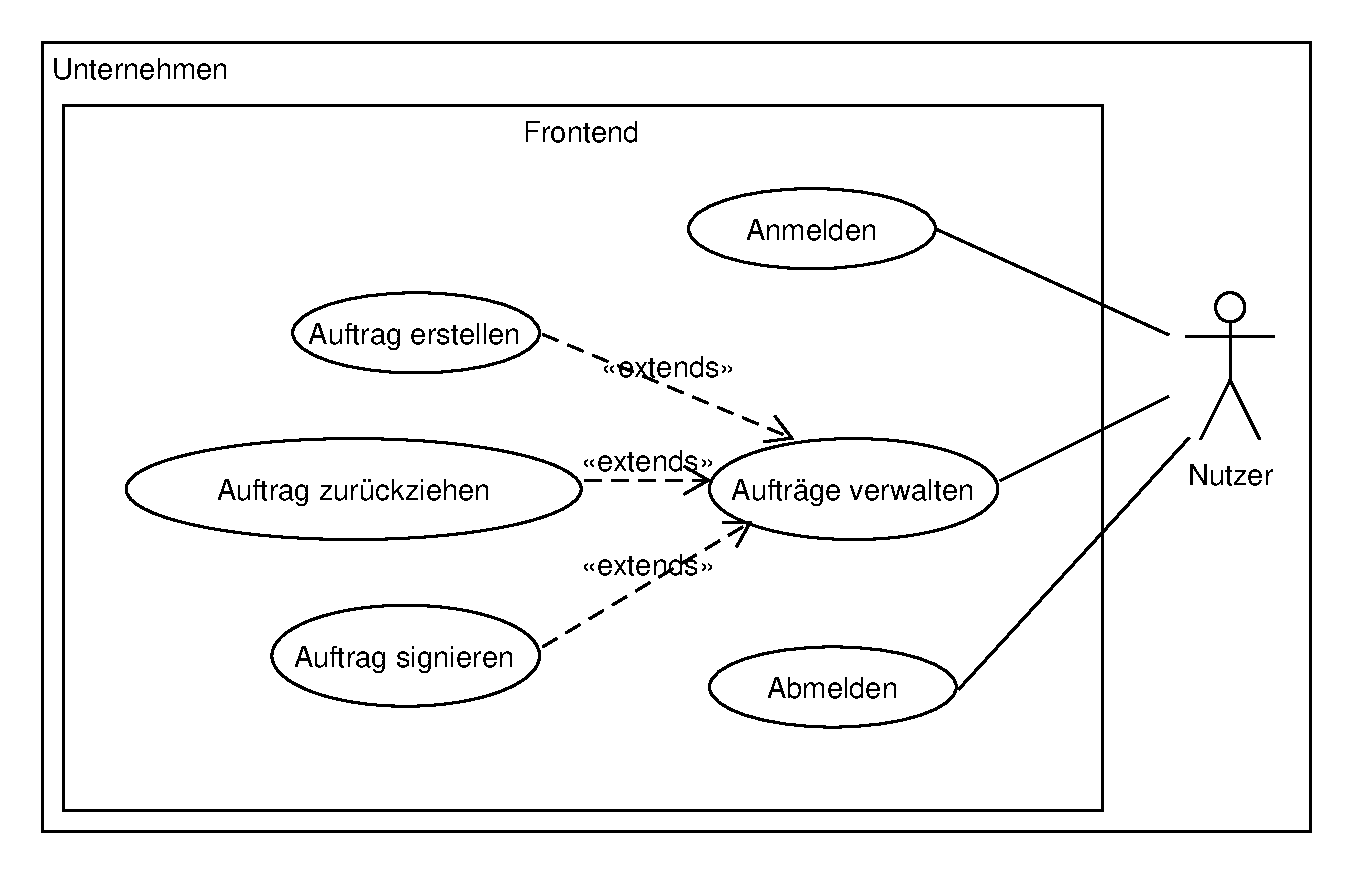
\includegraphics[width=1.0\textwidth]{UseCase_User.pdf}
	\caption{Aktionsübersicht des Nutzers}
	\label{fig:Bild2}
\end{figure}

\subsubsection{Szenario: Auftrag erstellen}
\paragraph{Beschreibung}
Nicolas möchte einen neuen Auftrag unter einem bestehenden Endpunkt für einen GUI-Entwurf einer Webseite, die Hundewelpen vermittelt, erstellen. Der GUI-Entwurf muss dafür von vier seiner Teamkollegen abgezeichnet werden.
\paragraph{Korrekter Ablauf}
Der Nutzer meldet sich am \gls{Frontend} an. Er wählt in der Auflistung der Endpunkte den Punkt \enquote{Zehn-Augen} aus. Er wird zur Erstellungsseite eines Auftrags für diesen Endpunkt weitergeleitet. Der Nutzer gibt folgende Konfiguration an:
\begin{itemize}
	\item Auftragsname: \enquote{Hundewelpen-Seite, GUI-Entwurf}.
	\item Signaturmodus: sequentiell
	\item Rollen: Wendy, Moritz, Noah, Julius (seine vier Teamkollegen)
	\item Benachrichtigung per E-Mail bei \gls{Status}änderung ist eingeschaltet.
\end{itemize}
\newpage
Er fügt den GUI-Entwurf als PDF-Datei hinzu. Dafür drückt er auf den \enquote{Datei hochladen}-Button und wählt seinen Entwurf im Dateiauswahldialog aus. Er bestätigt seine Konfiguration durch Klicken auf den \enquote{Auftrag erstellen}-Button. Nicolas wird zur Startseite des Frontends weitergeleitet und kann den erstellten Auftrag unter dem Punkt \enquote{Meine Aufträge} einsehen. Er erhält eine Bestätigungs-E-Mail mit allen Auftragsdetails.

\paragraph{Abgebrochener Ablauf}
Vor der Bestätigung durch den \enquote{Auftrag erstellen}-Button kann der Nutzer die Auftragserstellung an beliebiger Stelle abbrechen, indem er auf den \enquote{Abbrechen}-Button klickt oder das Fenster schließt.

\subsubsection{Szenario: Auftrag signieren}
\paragraph{Beschreibung}
Die Nutzer der Rolle \enquote{Personalabteilung} wurden per E-Mail benachrichtigt, dass ein neuer zu signierender Auftrag mit dem Betreff \enquote{Urlaubsantrag, Thomas Mayer} eingegangen ist. Ein Mitarbeiter der Personalabteilung kümmert sich um die Signierung des Auftrags.
\paragraph{Korrekter Ablauf}
Der Mitarbeiter der Personalabteilung meldet sich am Frontend an und wird auf die Startseite weitergeleitet. Durch Klicken auf den Menüpunkt \enquote{Zu signierende Aufträge} unter dem Reiter \enquote{Aufträge} kann er sich alle Aufträge auflisten lassen, die er mit seiner Rollen-Zugehörigkeit signieren kann. In der Auflistung der Aufträge klickt er auf den Auftrag \enquote{Urlaubsantrag, Thomas Mayer}. Er bekommt eine Detailansicht des Auftrags mit den folgenden Informationen zu sehen:
\begin{itemize}
	\item Fortschritt: noch nicht signiert
	\item Zugehörige Datei: Urlaubsantrag.pdf
	\item Anzahl der Augenpaare: vier
	\item Signaturmodus: sequentiell
	\item Signaturart: Button klicken
\end{itemize}
Der Mitarbeiter der Personalabteilung lädt sich die Datei \enquote{Urlaubsantrag.pdf} über den \enquote{Datei herunterladen}-Button herunter. Er prüft den Auftrag und signiert ihn, indem er auf den \enquote{Auftrag signieren}-Button klickt. Nach nochmaliger Bestätigung ist der Auftrag signiert.

\paragraph{Abgebrochener Ablauf}
Falls der Mitarbeiter das Fenster schließt, nicht auf den \enquote{Auftrag signieren}-Button drückt oder die Signatur des Auftrags nicht erneut bestätigt, wird die Signatur abgebrochen.

\section{Entwicklungsumgebung}
\subsection{Software}
\begin{table}[htbp]
    \begin{tabu} to \textwidth {| X | X |}
    \hline
    Betriebssysteme & Ubuntu \\
    \hline
    Textverarbeitung & \LaTeX \\
    \hline
    TeX-Distribution & TexLive \\
    \hline
    \LaTeX{-Editor} & Overleaf \\
    \hline
    \gls{UML}-Tool & Umlet\\
    \hline
    Design von \gls{Frontend}/\gls{Backend} & Notability \\
    \hline
    \gls{Python} Editor & Visual Studio Code \\
    \hline
    \gls{HTML} Editor & Visual Studio Code \\
    \hline
    \gls{JavaScript} Editor & Visual Studio Code \\
    \hline
    \gls{Versionskontrolle} & Git \\
    \hline
    Git \gls{Client} & Fork git-cli Visual Studio Code\\
    \hline
    \gls{Remote Repository} mit \gls{Continuous Integration} & Github (github.com) \\
    \hline
    Webserver Frontend/Backend & Django \\
    \hline
    Webserver \gls{REST-API} & Django \\
    \hline
    Skriptsprache für Webanwendungen & python \\
    \hline
    \gls{Datenbank} & postgresql \\
    \hline
    Datenbankadministration & TODO \\
    \hline
    Python-Paketmanager & pip \\
    \hline
    \gls{Webframework} Frontend/Backend & Django \\
    \hline
    Kommunikation im Team & Whatsapp Matrix Discord\\
    \hline
    \glslink{TLS}{TLS} \gls{Certificate Authority} & Let's Encrypt \\
    \hline
\end{tabu}
\end{table}

\subsection{Hardware}
Die Entwicklungsumgebung wird lokal unter Windows, MacOS und Linux entwickelt, jedoch wird es in der Produktion nur auf Linux Servern laufen. Die Systemanforderungen werden möglichst gering gehalten um mögliche Hardware Änderungen ohne Umstellungen vornehmen zu können.
Weitere Infrastruktur wird für den Einsatz von \name nicht benötigt.
\section{Glossar}

% Automatisch generiertes Glossar (Latex zwei mal ausführen um Glossar anzuzeigen)
%\glsaddall % das sorgt dafür, dass alles Glossareinträge gedruckt werden, nicht nur die verwendeten. Das sollte nicht nötig sein!
\printnoidxglossaries
\section{Anhang}

\subsection{Frontend}
\begin{figure}[!htb]
	\centering
	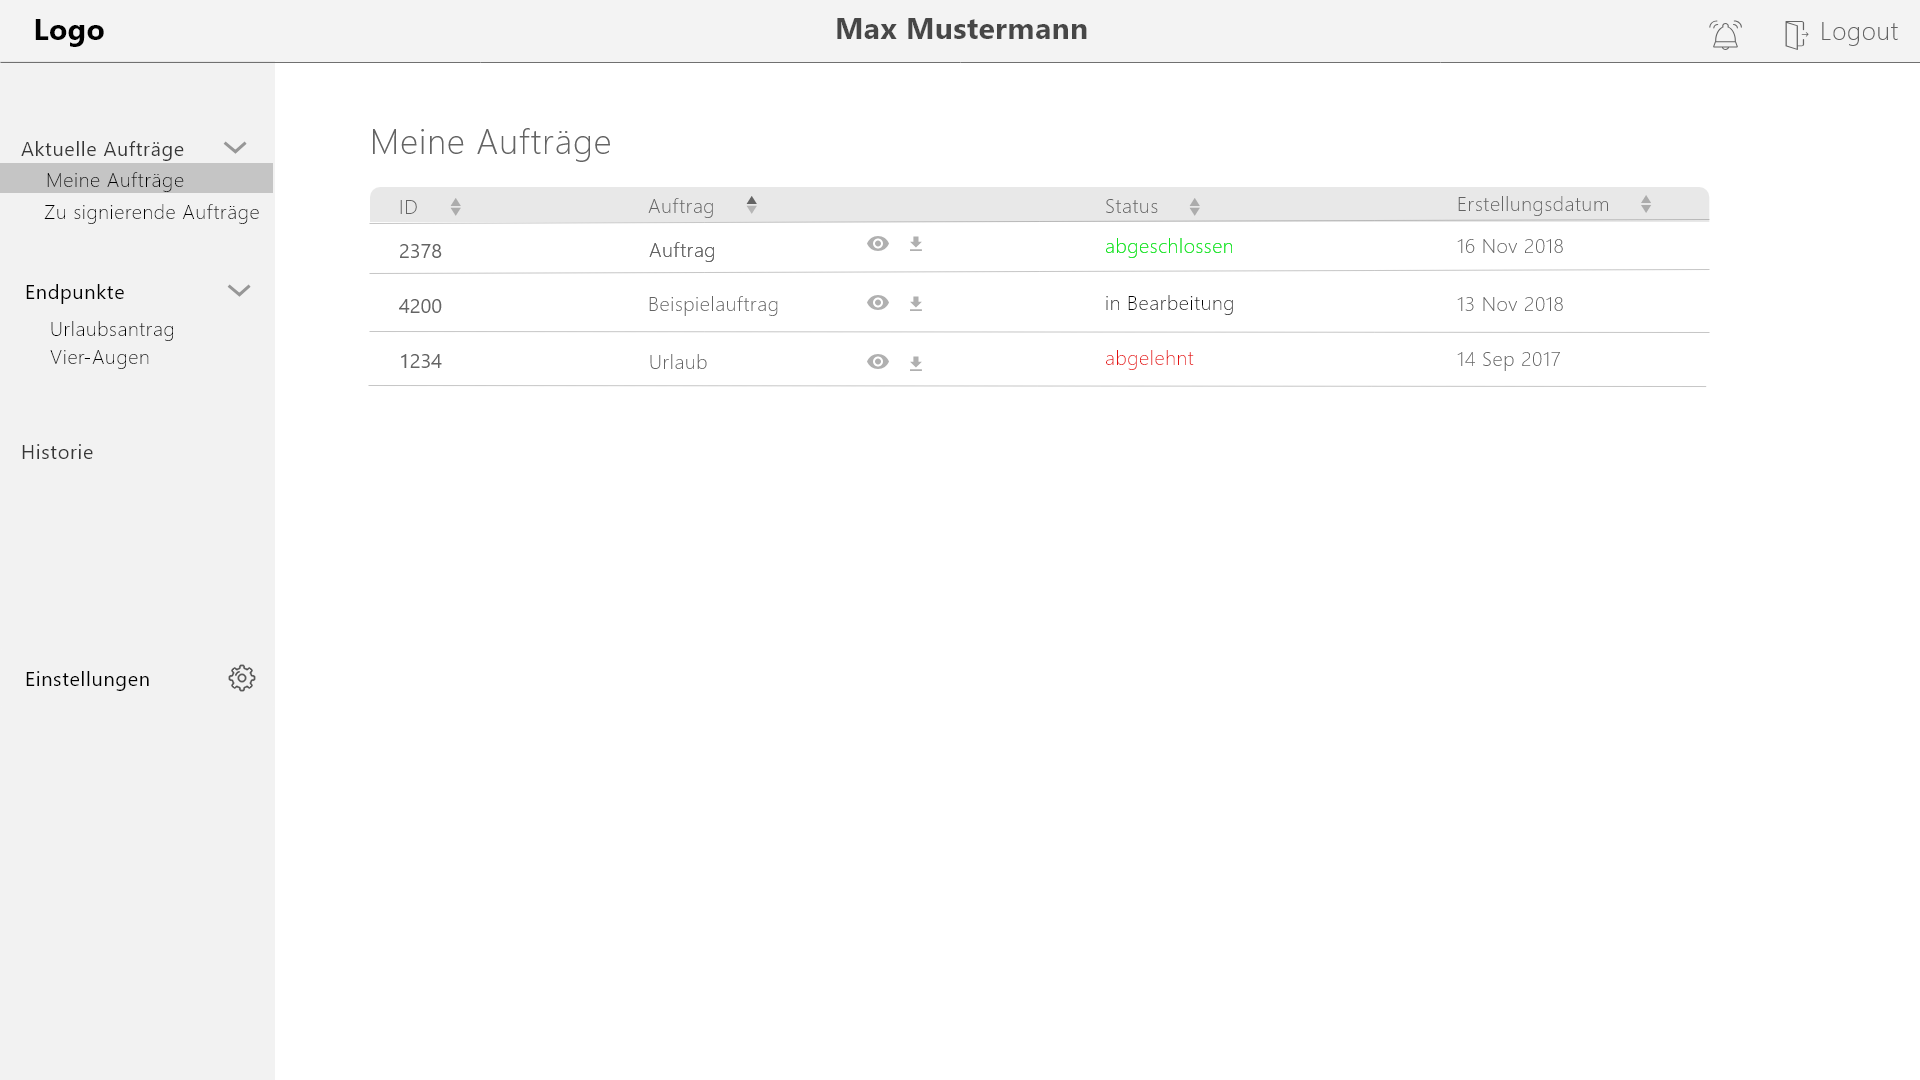
\includegraphics[width=\textwidth]{Nutzer-Startseite.png}
	\caption{Startseite des Nutzers}
\end{figure}
\vspace{1.5cm}
\begin{figure}[!htb]
	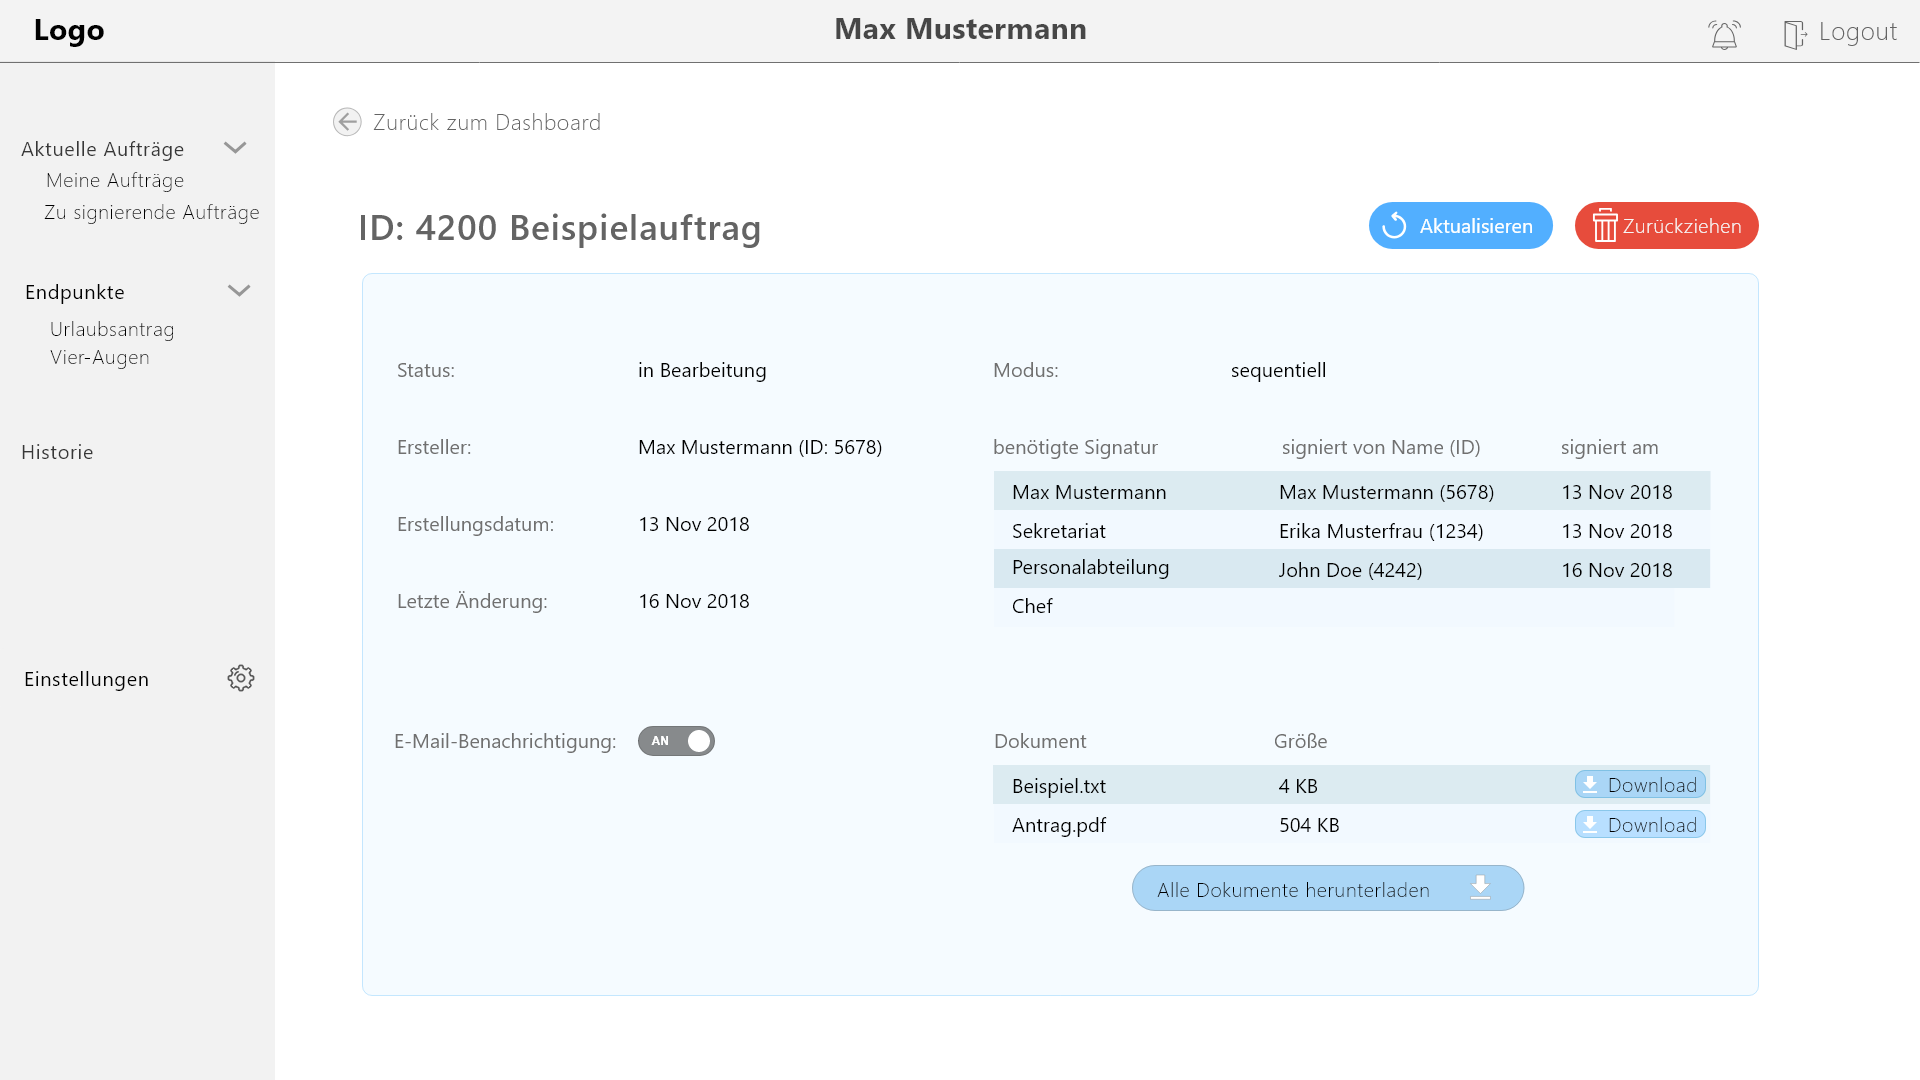
\includegraphics[width=\textwidth]{Auftrag-Detailansicht.png}
	\caption{Detailsicht eines selbst erstellten Auftrags}
\end{figure}

\newpage
\subsection{Backend}
\begin{figure}[!htb]
	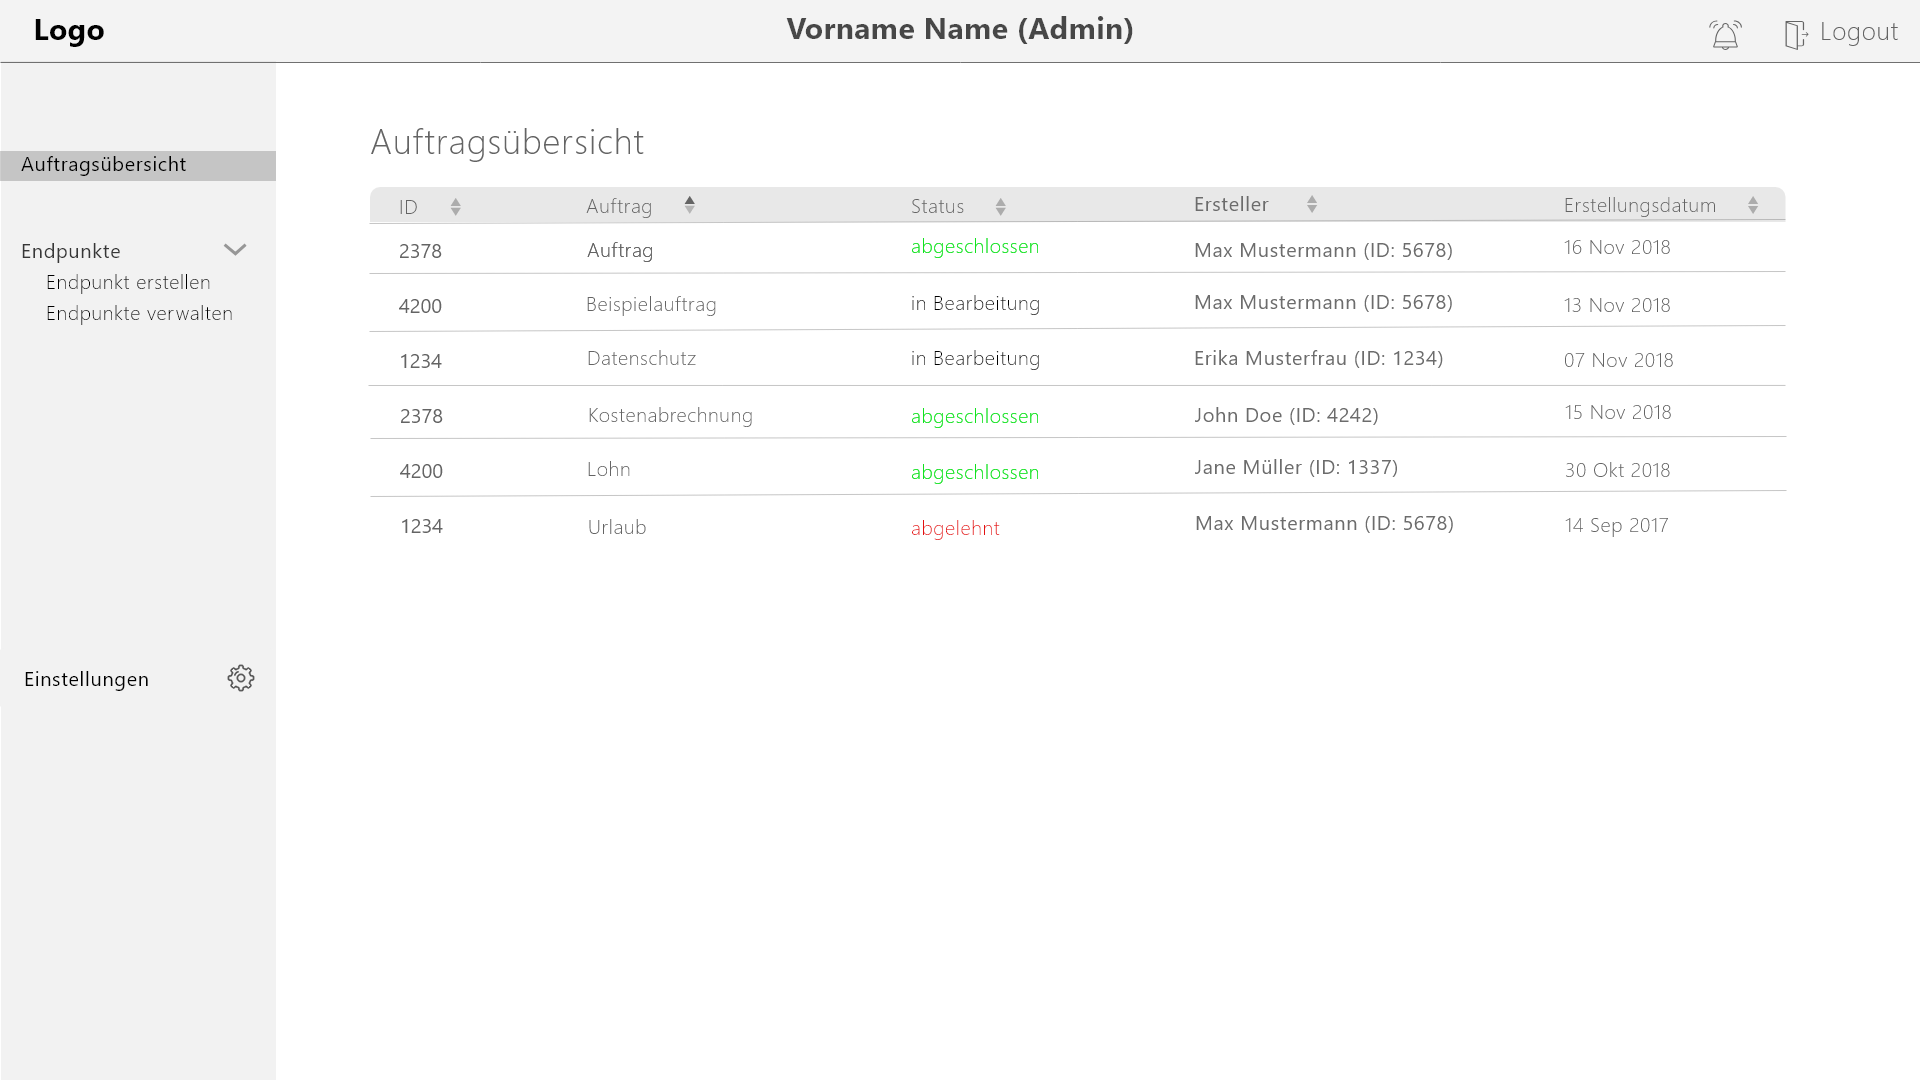
\includegraphics[width=\textwidth]{Admin-Uebersicht.png}
	\caption{Admin-Übersicht}
\end{figure}
\vspace{1.5cm}
\begin{figure}[!htb]
	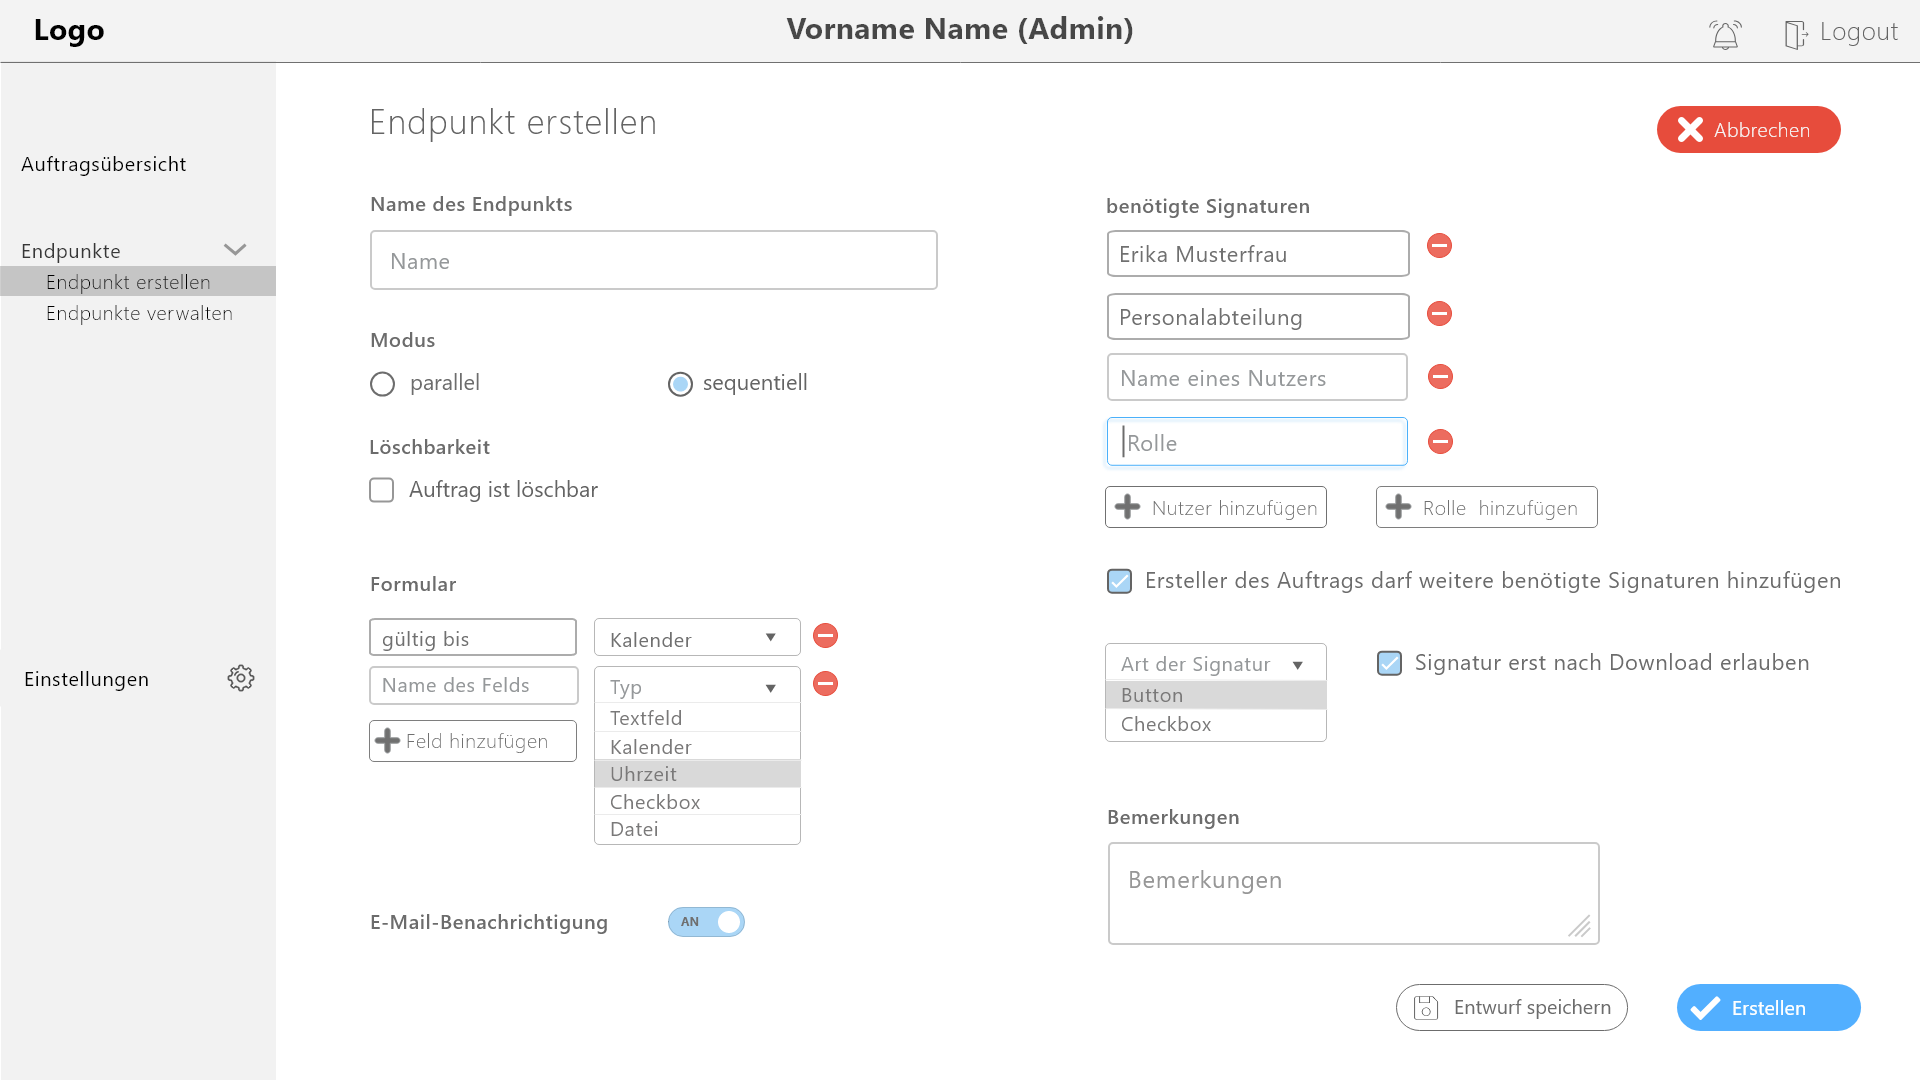
\includegraphics[width=\textwidth]{Endpunkt-Erstellen.png}
	\caption{Ansicht bei Erstellung eines Endpunkts}
\end{figure}

% end content
\end{document}